\documentclass[a4paper,11pt]{article}

\usepackage[utf8]{inputenc}

\usepackage{graphicx}
\usepackage{caption}
\usepackage{subcaption}

\usepackage{pgfplots}
\pgfplotsset{compat=1.18} 

\usepackage{minted}
\usepackage{siunitx}

\begin{document}

\title{
    \textbf{Trees in C}
}
\author{Mo Wang}
\date{Spring 2026}

\maketitle

\section*{Introduction}

This report examines the performance and behavior of binary trees in C. A binary tree is a linked data structure that begins from the root node and stores two pointers to two other nodes, each of which in turn branches into two additional nodes. Ultimately nodes that do not divide to additional node branches are called leaf nodes. Conceptually, the tree is drawn from the root node on top, whereas it branches downward towards the leaf nodes. Each node branches into a left and a right node.

\section*{Structural implementation of a binary tree}

A binary tree can be created using two different structures: one node block that stores its integer value and the pointer address to two other nodes, and a tree control block that stores the address of the root node. A leaf node holds two null pointers in the left and right node entries.

\begin{minted}{c}
typedef struct node {
    int value;
    struct node *right;
    struct node *left;
} node;

typedef struct tree {
    node *root;
} tree;
\end{minted}

A node can be constructed by allocating it inside a tree, which can be done by dynamically allocating memory for the node and initializing its value. Similarly, the tree control block can also be constructed in this pattern.

\begin{minted}{c}
node *construct_node(int val) {
    node *nd = (node*) malloc(sizeof(node));
    nd->value = val;
    nd->left = NULL;
    nd->right = NULL;
    return nd;
}

void free_node(node *nd) {
    // Freeing the nodes could be done recursively.
    if (nd != NULL) {
        free_node(nd->left);
        free_node(nd->right);
        free(nd);
    }
}

tree *construct_tree() {
    tree *tr = (tree*) malloc(sizeof(tree));
    tr->root = NULL;
    return tr;
}

void free_tree(tree *tr) {
    if (tr != NULL){
        free_node(tr->root);
        free(tr);
    }
}
\end{minted}

Freeing a node is not as straightforward as creating one, because it contains pointer addresses to other nodes, which would be lost in memory leakage if the node is simply removed. To address this, when a node is freed, the operation ensures that all nodes it points to are also freed. The \texttt{free\_node} function recursively frees the nodes, starting from a given node, while \texttt{free\_tree} function de-allocates the tree control block alongside with all of its nodes, both functions ensuring no memory leakage is caused.

\section*{Operations of a sorted binary tree}

One special case of a binary tree is the sorted binary tree, which efficiently maintains a sorted order of a group values. In this case, integers are used as values, since they can be easily compared using less-than and greater-than operators. In a sorted binary tree, the left sub-tree branch of a node holds integers that are less than the integer value of the node itself, while the right branch holds integers larger than the value of the node. This structure creates an implicitly sorted sequence of integers beginning from the leftmost node of the tree to the rightmost one.

Binary sorted tree operations involve inserting an integer value into the tree as well as searching for a certain integer value, while maintaining the sorted sequence order inside the tree.

\subsection*{Add operation}

An insertion operation can be implemented recursively by beginning from the root node and comparing the insertion value to its current node value. If the insertion value is equal to the node value, no insertion operation is performed, as duplicated values are not allowed. However, if the inserted value is less than the node value, the left node will be proceeded, otherwise, the right node will be traversed, where the process starts over. As the leaf node is reached, the value is attached to the suitable branch, either left or right depending on the leaf node value.

\begin{minted}{c}
node* add_node(node *nd, int value){
    // helper function (recursive)
    if (nd == NULL){
        return construct_node(value);
    }
    if (value < nd->value){
        nd->left = add_node(nd->left, value);
    }
    else if (value > nd->value){
        nd->right = add_node(nd->right, value);
    }
    return nd;
}

void recursive_add(tree *tr, int value){
    // recursive
    tr->root = add_node(tr->root, value);
}
\end{minted}

\subsubsection*{Theoretical time complexity}

The time complexity is proportional to the depth of the tree, since the algorithm has to traverse down to the leaf node before a value can be attached. The depth can vary in different cases. The best case is a fully balanced tree with $n$ nodes, resulting into $\log_2(n)$ depth and logarithmic time complexity $O(\log_2(n))$. However, in the worst case, the tree can degenerate into a linked list with $n$ depth, resulting in linear time complexity $O(n)$.

\subsubsection*{Add operation without recursion}

The insert operation can also be implemented without recursion. In this case, traversal down each depth level can be maintained by current node variable \texttt{nd} and parent node variable \texttt{parent}. The algorithm starts from the root node and traverses the tree by comparing the insertion value with the current node value. Depending on the value being smaller or larger than the insertion value, the algorithm moves to left or right child, updating both \texttt{parent} and \texttt{nd} variables, until an appropriate leaf node is reached. At that point, the new node is attached as a left or right child, depending on the value of the parent node.

Since the non-recursive implementation omits function call and additional stack frame push on each depth traversal, the performance, both time and space, is generally better than recursive implementation, given the same binary tree.

\begin{minted}{c}
void add(tree *tr, int value){
    node* parent = NULL;
    node* nd = tr->root;
    while (nd != NULL){
        parent = nd;
        if (value < nd->value)
            nd = nd->left;
        else if (value > nd->value)
            nd = nd->right;
        else
            return;
    }
    node* new_node = construct_node(value);
    if (parent == NULL){
        tr->root = new_node;
        return;
    }
    if (value < parent->value)
        parent->left = new_node;
    else
        parent->right = new_node;
}
\end{minted}

\subsection*{Lookup procedure}

The lookup procedure can, in the simplest form, be implemented with recursion. In each tree depth traversal, the search value is compared with the node value. If the value is the same as the node value, the value is already found. Otherwise, depending on whether the search value is smaller or greater than the node’s value, the procedure is recursively repeated in the left or right sub-tree, respectively, until the leaf node is reached to decide whether the value exists in the tree.

\begin{minted}{c}
bool lookup_node(node *nd, int value){
    if (nd == NULL) return false;
    if (value < nd->value) return lookup_node(nd->left, value);
    else if (value > nd->value) return lookup_node(nd->right, value);
    return true;
}

bool recursive_lookup(tree *tr, int value){
    return lookup_node(tr->root, value);
}
\end{minted}

\subsubsection*{Theoretical time complexity}

Since the algorithm traverses the tree down to the leaf node in order to find a target value, the time complexity is in maximum proportional to the depth of the tree. The tree depth usually varies with different sets of integers. In the best case, the depth is roughly 2-logarithm of the number of nodes in the tree $\log_2(n)$, where the tree is relatively balanced. However, in the worst case, the tree can become left- or right-heavy and degenerate to a linked list, where the depth of the tree is equal to the tree size $n$. So, the time complexity is logarithmic $O(\log_2(n))$ in the best case, while in the worst case, it can degrade to linear time complexity $O(n)$.

\subsubsection*{Benchmark}

To evaluate the theoretical time complexity in practice, lookup operation is benchmarked while its input size increases. In the first benchmark, during insertion, the sorted binary tree is constructed by successively inserting numbers from a shuffled continuous sequence to the tree, while benchmarking the minimal time. The growth trend is slightly less than linear time complexity, which can be visualized as lookup BST shuffled in Table~\ref{tab:bst-lookup-complexity} and correspond to the green curve in Figure~\ref{fig:bst-lookup-complexity}. The non-logarithmic time complexity during insertion a shuffled continuous sequence is mostly because that the tree may not always be balanced. In some pathological cases, the tree can be relatively unbalanced, which causes longer depth and more performance overhead.


\begin{table}[h]
  \centering
  \begin{tabular}{r|r|r|r}
    \textbf{N} & \textbf{lookup\_BST\_balanced} & \textbf{lookup\_BST\_shuffled} & \textbf{lookup\_BST\_unbalanced} \\ \hline
     1024   &     29\,370    &     30\,725    &      34\,553    \\
     2048   &     93\,654    &     97\,052    &     110\,181    \\
     4096   &    531\,565    &    569\,464    &     588\,317    \\
     8192   &  1\,503\,405    &  1\,590\,799    &   1\,613\,613    \\
    16384   &  3\,150\,780    &  3\,232\,780    &   3\,522\,417    \\
    32768   &  5\,626\,569    &  5\,781\,768    &   5\,801\,364    \\
    65535   &  8\,979\,048    &  10\,318\,486    &  11\,077\,433    \\
   131072   & 11\,818\,138    &  19\,596\,716    &  23\,315\,456    \\
  \end{tabular}
  \caption{Balanced vs shuffled vs unbalanced BST lookup times (ns).}
  \label{tab:bst-lookup-complexity}
\end{table}

\begin{figure}[h]
  \centering
  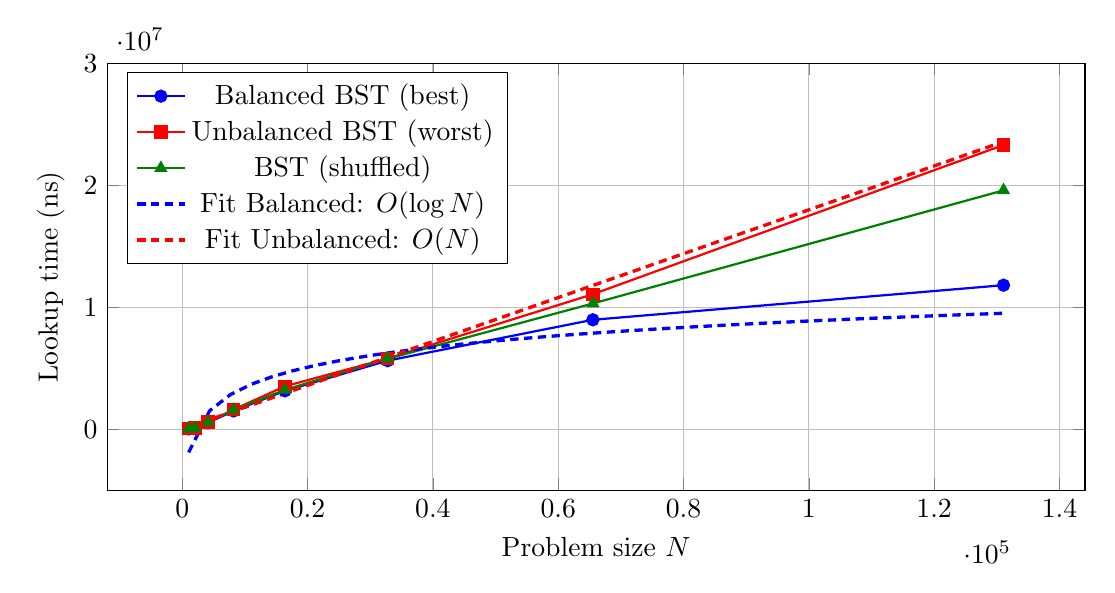
\begin{tikzpicture}
    \begin{axis}[
      % xmode=log, ymode=log,
      xlabel={Problem size $N$},
      ylabel={Lookup time (ns)},
      width=14cm, height=7cm,
      grid=major,
      legend style={at={(0.02,0.98)}, anchor=north west, draw=black, fill=white},
      xmajorgrids=true, ymajorgrids=true,
      ymin=-0.5e7, ymax=3e7
    ]

      % -------------------------------
      % Balanced BST (measured)
      % -------------------------------
      \addplot[
        color=blue,
        mark=*,
        thick
      ] coordinates {
        (1024,29370)
        (2048,93654)
        (4096,531565)
        (8192,1503405)
        (16384,3150780)
        (32768,5626569)
        (65535,8979048)
        (131072,11818138)
      };
      \addlegendentry{Balanced BST (best)}

      % -------------------------------
      % Unbalanced BST (measured)
      % -------------------------------
      \addplot[
        color=red,
        mark=square*,
        thick
      ] coordinates {
        (1024,34553)
        (2048,110181)
        (4096,588317)
        (8192,1613613)
        (16384,3522417)
        (32768,5801364)
        (65535,11077433)
        (131072,23315456)
      };
      \addlegendentry{Unbalanced BST (worst)}

      % -------------------------------
      % Shuffled-input BST (measured)
      % -------------------------------
      \addplot[
        color=green!50!black,
        mark=triangle*,
        thick
      ] coordinates {
        (1024,30725)
        (2048,97052)
        (4096,569464)
        (8192,1590799)
        (16384,3232780)
        (32768,5781768)
        (65535,10318486)
        (131072,19596716)
      };
      \addlegendentry{BST (shuffled)}

      % -----------------------------------------
      % Fitted O(log N) line (Balanced tree)
      % -----------------------------------------
      \addplot[
        blue,
        densely dashed,
        very thick,
        domain=1024:131072,
        samples=40
      ] {1.63e6 * (ln(x)/ln(2)) - 1.82e7};
      \addlegendentry{Fit Balanced: $O(\log N)$}

      % -----------------------------------------
      % Fitted O(N) line (Unbalanced tree)
      % -----------------------------------------
      \addplot[
        red,
        densely dashed,
        very thick,
        domain=1024:131072,
        samples=40
      ] {180 * x};
      \addlegendentry{Fit Unbalanced: $O(N)$}

    \end{axis}
  \end{tikzpicture}

  \caption{Balanced vs unbalanced vs shuffled‑input BST lookup: logarithmic vs linear growth.}
  \label{fig:bst-lookup-complexity}
\end{figure}

To calculate the range of complexity of binary search tree lookup operation, two extreme cases of a binary tree are taken into consideration: a fully balanced binary tree with 2-logarithmic time complexity $O(\log(n))$, visualized in Figure~2(a), as well as a fully unbalanced tree where an ordered sequence of values is inserted into an empty tree, degenerating into a linked list with linear time complexity $O(n)$, shown in Figure~2(b) with all right children. Benchmark statistics show that the fully balanced tree serves as the lower boundary for execution time, while the most heavily unbalanced tree represents the upper boundary, as shown in Figure~1. The average case, with a shuffled sequence of numbers, lies between these two extremes.

\begin{figure}[h]
  \centering

  %-------------------- Left: Balanced --------------------
  \begin{subfigure}[t]{0.48\textwidth}
    \centering
    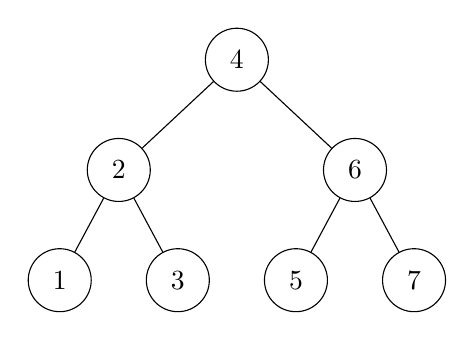
\begin{tikzpicture}[
        level distance=1.4cm,
        every node/.style={circle,draw,minimum size=8mm},
        level 1/.style={sibling distance=30mm},
        level 2/.style={sibling distance=15mm}
    ]
    \node {4}
        child { node {2}
            child { node {1} }
            child { node {3} }
        }
        child { node {6}
            child { node {5} }
            child { node {7} }
        };
    \end{tikzpicture}
    \subcaption{Balanced binary tree}
    \label{fig:balanced}
  \end{subfigure}
  \hfill
  %-------------------- Right: Unbalanced --------------------
  \begin{subfigure}[t]{0.48\textwidth}
    \centering
    \begin{tikzpicture}[
        level distance=1cm,
        every node/.style={circle,draw,minimum size=8mm},
        level 1/.style={sibling distance=25mm},
        level 2/.style={sibling distance=25mm},
        level 3/.style={sibling distance=25mm},
    ]
    \node {1}
      child [missing]
      child { node {2}
        child [missing]
        child { node {...}
          child [missing]
          child { node {7} }
        }
      };
    \end{tikzpicture}
    \subcaption{Fully unbalanced (all right children)}
    \label{fig:unbalanced}
  \end{subfigure}

  \caption{Balanced vs unbalanced binary trees placed side by side.}
  \label{fig:balanced-vs-unbalanced}
\end{figure}

\subsubsection*{Comparison with binary search algorithm}

Both lookup operation in binary sorted tree and binary search algorithm in array is similar in terms of algorithm, but they produce different behavior during runtime performance, due to different data structures.

The search operation in the binary sorted tree has a time complexity of $O(\log(n))$, in the best case, which occurs when the tree is balanced with depth $\log_2(n)$. In this case, the runtime behavior is similar to that of the binary search algorithm on an array, as both involve splitting the sequence in half and recursively selecting the relevant half. However, searching in a binary search tree introduces a slight overhead due to constant pointer chasing and potential cache thrashing, which does not occur with binary search on an array. In Table~\ref{tab:bst-binary-search-complexity}, binary search algorithm slightly outperforms lookup operation in binary search trees (BST) in large number of integer values which can also be visualized in Figure~\ref{fig:bst-binary-search-complexity}.

\begin{table}[h]
  \centering
  \begin{tabular}{r|r|r}
    \textbf{N} & \textbf{lookup\_ns(BST)} & \textbf{lookup\_ns(binsearch)} \\ \hline
     1024   &        29\,370  &        54\,047   \\
     2048   &        93\,654  &       127\,333   \\
     4096   &       531\,565  &       595\,292   \\
     8192   &     1\,503\,405  &     1\,515\,735   \\
    16384   &     3\,150\,780  &     3\,185\,937   \\
    32768   &     5\,626\,569  &     5\,555\,768   \\
    65535   &     8\,979\,048  &     8\,551\,890   \\
   131072   &    11\,818\,138  &    11\,092\,376   \\
  \end{tabular}
  \caption{Lookup times (ns) for BST and array binary search (new results).}
  \label{tab:bst-binary-search-complexity}
\end{table}

% Preamble:
% \usepackage{pgfplots}
% \pgfplotsset{compat=1.18}

\begin{figure}[h]
  \centering
  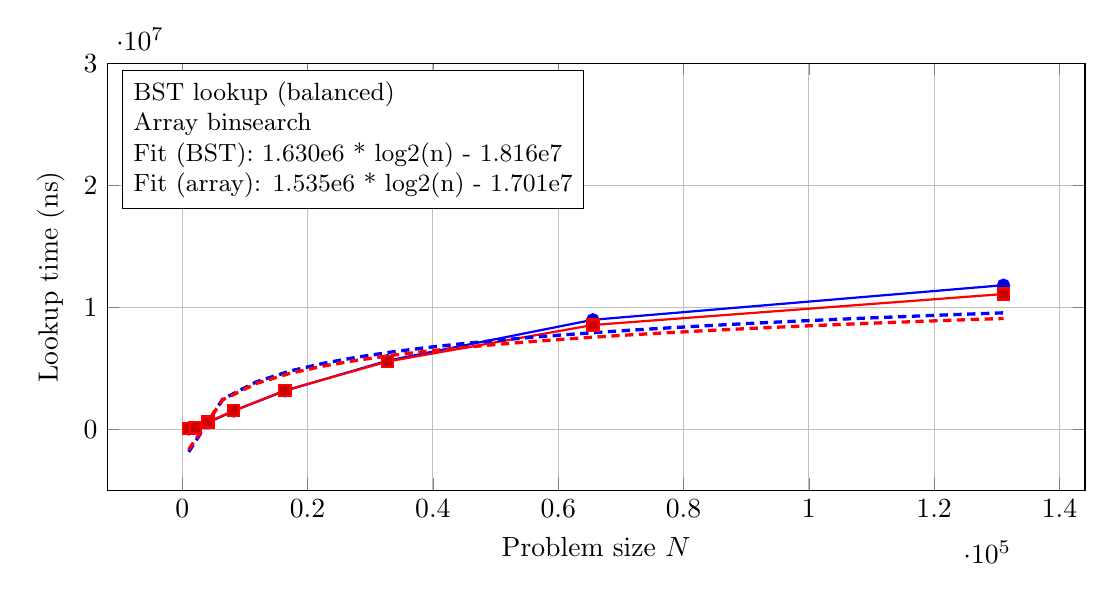
\begin{tikzpicture}
    \begin{axis}[
      xlabel={Problem size $N$},
      ylabel={Lookup time (ns)},
      width=14cm, height=7cm,
      grid=major,
      ymajorgrids=true,
      xmajorgrids=true,
      clip=true,
      ymin=-0.5e7, ymax=3e7
    ]

      % ----------------------------------------------------------------
      % Measured data: BST (new results)
      % ----------------------------------------------------------------
      \addplot+[
        mark=*,
        thick,
        color=blue
      ] coordinates {
        (1024,     29370)
        (2048,     93654)
        (4096,    531565)
        (8192,   1503405)
        (16384,  3150780)
        (32768,  5626569)
        (65535,  8979048)
        (131072,11818138)
      };

      % ----------------------------------------------------------------
      % Measured data: Array binsearch (new results)
      % ----------------------------------------------------------------
      \addplot+[
        mark=square*,
        thick,
        color=red
      ] coordinates {
        (1024,     54047)
        (2048,    127333)
        (4096,    595292)
        (8192,   1515735)
        (16384,  3185937)
        (32768,  5555768)
        (65535,  8551890)
        (131072,11092376)
      };

      % ----------------------------------------------------------------
      % Fitted O(log2 N) line for BST (full span; fast sampling)
      %   a = 1.629534e6,  b = -1.815714e7  (least-squares on log2(N))
      % ----------------------------------------------------------------
      \addplot[
        blue,
        densely dashed,
        very thick,
        domain=1024:131072,
        samples=25
      ] {1.6295341135e6 * (ln(x)/ln(2)) - 1.8157139922690175e7};

      % ----------------------------------------------------------------
      % Fitted O(log2 N) line for Array (full span; fast sampling)
      %   a = 1.535034e6,  b = -1.701316e7  (least-squares on log2(N))
      % ----------------------------------------------------------------
      \addplot[
        red,
        densely dashed,
        very thick,
        domain=1024:131072,
        samples=25
      ] {1.5350338421e6 * (ln(x)/ln(2)) - 1.7013155393798765e7};

      % ----------------------------------------------------------------
      % In-figure boxed note — NOW TOP-LEFT
      % rel axis cs: (0,0)=bottom-left; (1,1)=top-right
      % ----------------------------------------------------------------
      \node[anchor=north west, draw=black, fill=white,
            inner sep=4pt, align=left, font=\small]
           at (rel axis cs: 0.015, 0.985)
           {BST lookup (balanced)\\
            Array binsearch\\
            Fit (BST): 1.630e6 * log2(n) - 1.816e7\\
            Fit (array): 1.535e6 * log2(n) - 1.701e7};

    \end{axis}
  \end{tikzpicture}
  \caption{Lookup benchmark (new results): BST vs array binary search with $O(\log_2 N)$ fits; legend box placed in the top-left.}
  \label{fig:bst-binary-search-complexity}
\end{figure}


As the tree becomes unbalanced, the time complexity degrades towards $O(n)$, as the depth level approaches the number of elements in the array $n$. In contrast, the binary search on the sorted array remains unaffected by structural imbalance, consistently maintaining a time complexity of $O(\log(n))$. Thus, the binary search in an array generally outperforms the binary search algorithm in an unbalanced binary search tree.

\section*{Depth first traversal}

... Depth-first traversal -> you go down as deep as possible before considering the alternatives. called in-order ( The item of the node is thus in-between the items of the left and the right branch.) -> natural sorted order
We could also present the items in a pre-order or post-order; the name describes where in the order we place the item of the node.

\begin{minted}{c}
static void print(node *nd) {
    if (nd != NULL) {
        print(nd->left);
        printf("%d ", nd->value);
        print(nd->right);
    }
}
void print_tree(tree *tr) {
    if (tr->root != NULL)
        print(tr->root);
    printf("\n");
}
\end{minted}

\section*{Traversal using explicit stack}

Explicit stack: (implement the print method)
Use your dynamic stack implementation from one of the first assignments and adapt it to be a stack of nodes (pointers to nodes).
Invariant: The left sub-tree of a node that is pop:ed from the stack has been printed, the value of the node itself has not, nor the values of the right sub-tree.

\texttt{static stack *stack\_create()}, \texttt{static void stack\_free(stack *stk)}, \texttt{static void stack\_push(stack *stk, node *nd)}, \texttt{static bool stack\_empty(const stack *stk)}, \texttt{static node *stack\_pop(stack *stk)}

\begin{minted}{c}
void tree_print_inorder_stack(const tree *tr) {
    stack *stk = stack_create();
    node *nd = tr->root;

    /* move to leftmost path initially */
    while (nd != NULL) {
        stack_push(stk, nd);
        nd = nd->left;
    }

    while (!stack_empty(stk)) {
        node *nd = stack_pop(stk);
        printf("%d ", nd->value);  /* left handled, now visit node */

        /* then handle right subtree: push its left path */
        node *r = nd->right;
        while (r != NULL) {
            stack_push(stk, r);
            r = r->left;
        }
    }
    stack_free(stk);
    printf("\n");
}
\end{minted}

... Implement the print procedure and test it to see that it works. You might wonder if there is any reason to use an explicit stack instead of the stack of the programming language but it turns out that it could come in handy. In the print example there is no point in using an explicit stack but we could have a scenario where we want to save a state that describes the sequence of elements after a specific element; more on this on a lecture.

\section*{Conclusion}

... To sum up, ... the raw implementation of a linked-list queue maintains only a pointer to the first element, which forces each \texttt{enqueue} operation to traverse the entire list. This results in linear time complexity $O(n)$ for placing an element in a queue, which is attached to the end of the list. By extending the structure with an additional pointer to the last element, the improved queue can access the last element directly and attach new elements in the tail, which reduces the time complexity from linear order $O(n)$ to constant order $O(1)$. The performance results conform with the theoretical expectation and clearly visualize the performance improvement, where the enqueue time complexity becomes independent of queue size in the order of a random access, while the dequeue operation remains constant time complexity (see table~4).

\begin{table}[h]
\centering
\begin{tabular}{l|c|c}
\textbf{Operation} 
    & \textbf{Raw queue (head-only)} 
    & \textbf{Improved queue (head+tail)} \\ \hline
Enqueue complexity 
    & $O(n)$ 
    & $O(1)$ \\ \hline
Dequeue complexity
    & $O(1)$ 
    & $O(1)$ \\ \hline
\end{tabular}
\caption{Comparison of raw queue and improved queue performance}
\label{tab:queue-performance-comparison}
\end{table}

\end{document}